\begin{figure}[!htb]
    \centering
    \centering
    \begin{subfigure}{0.48\linewidth}
        \centering
        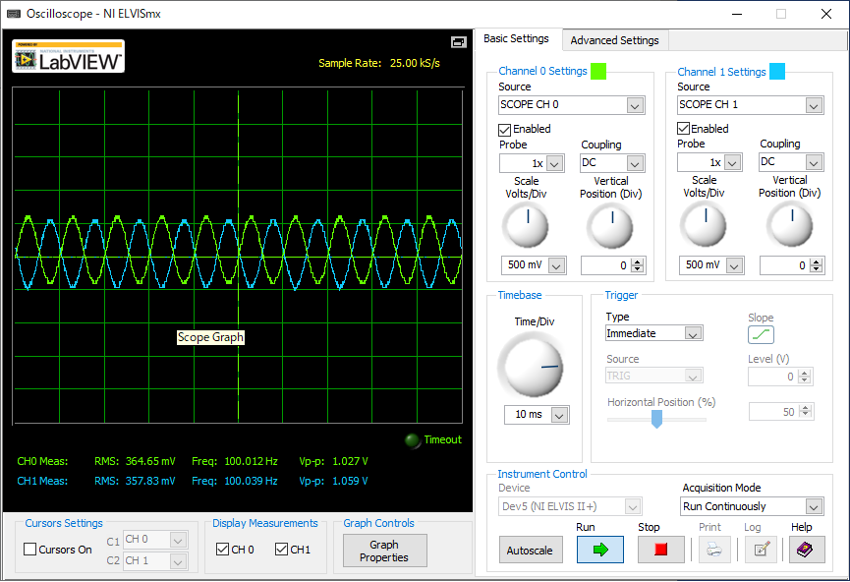
\includegraphics[width=0.8\linewidth]{src/figures/exp5/amp-10k.png}
        \subcaption{$R=\SI{10}{k\ohm}$のとき}\label{fig:exp5-raw-10k}
    \end{subfigure}
    \begin{subfigure}{0.48\linewidth}
        \centering
        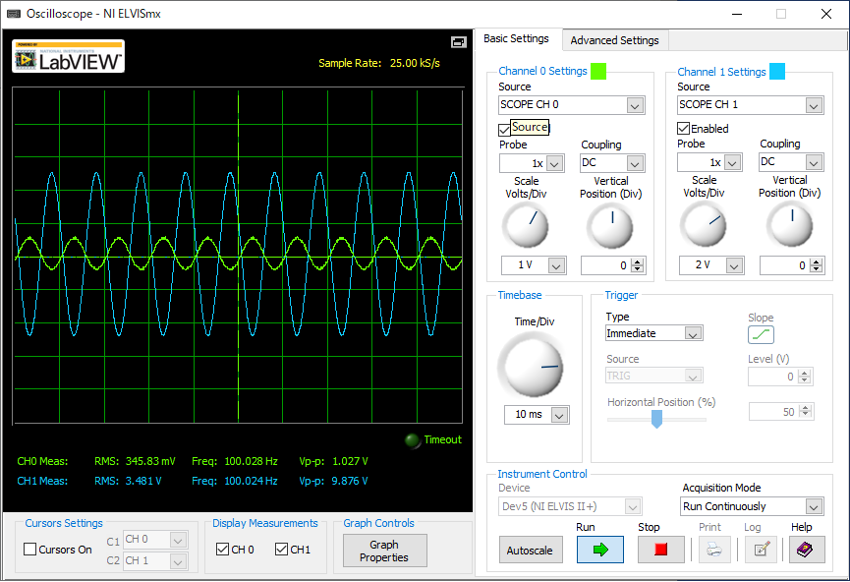
\includegraphics[width=0.8\linewidth]{src/figures/exp5/amp-1k.png}
        \subcaption{$R=\SI{1}{k\ohm}$のとき}\label{fig:exp5-raw-1k}
    \end{subfigure}
    \caption{実験5 オペアンプの出力波形}\label{fig:exp5-raw}
\end{figure}
